\documentclass[a4paper]{article}
\usepackage{graphicx} % Required for inserting images
\usepackage{amssymb}
\usepackage{amsmath}
\usepackage{hyperref}
\usepackage{listings}
\usepackage{fancyhdr}
\usepackage{xcolor}
\usepackage{geometry}
\usepackage{ragged2e}
\usepackage{subcaption}
\usepackage{multirow}
\usepackage{tabularx}
\usepackage{indentfirst}
\usepackage{lscape}
\usepackage{titlesec}
\usepackage[nottoc,numbib]{tocbibind}
\usepackage[usenames, dvipsnames]{xcolor}
\usepackage{tikz} \usetikzlibrary{calc}


\geometry{margin=1in}

\colorlet{myGreen}{green!70!black}
\colorlet{myDGreen}{green!50!black}
\colorlet{myGray}{white!60!black}

\newcommand{\colNaN}[1]{{\textcolor{black!30}{#1}}}
\newcommand{\colDisaster}[1]{{\textcolor{red!60}{#1}}}
\newcommand{\colFailure}[1]{{\textcolor{orange}{#1}}}
\newcommand{\colWorse}[1]{\textcolor{orange!60}{#1}}
\newcommand{\colSimilar}[1]{\textcolor{black!60}{#1}}
\newcommand{\colBetter}[1]{\textcolor{blue!70}{#1}}
\newcommand{\colSuccess}[1]{\textcolor{black!30!green}{#1}}
\newcommand{\colAmazing}[1]{\textcolor{green}{#1}}

\hypersetup{
    colorlinks,
    linkcolor={blue!50!black},
    citecolor={blue!50!black},
    urlcolor={blue!80!black}
}

\lstdefinestyle{mystyle}{
    language=Python,
    backgroundcolor=\color{white!95!black},   
    %commentstyle=\color{},
    %keywordstyle=\color{},
    %numberstyle=\tiny\color{codegray},
    %stringstyle=\color{codepurple},
    basicstyle=\ttfamily\footnotesize,
    breakatwhitespace=false,         
    breaklines=true,                 
    %captionpos=b,                    
    keepspaces=true,                 
    %numbers=left,                    
    %numbersep=5pt,                  
    showspaces=false,                
    showstringspaces=false,
    showtabs=false,                  
    tabsize=4,
}
\lstset{
    style=mystyle,
    %emph={sage},
    %emphstyle={\color{myGreen}}
}



%\renewcommand\footnoterule{\rule{.4\textwidth}{0.2pt}}
\renewcommand\footnoterule{\kern-3pt \hrule  \kern 2.6pt}
\fancyhead[L, C]{}
\fancyfoot[C]{\thepage}
\pagestyle{fancy}

\title{Internship report}
\author{Marie BONBOIRE}
\date{}

\begin{document}

\thispagestyle{plain}
\begin{titlepage}
    \begin{figure}[h]
        \centering
        
\includegraphics[width=0.4\textwidth]{su.png}
    \end{figure}
    \vspace{1cm}

    \begin{center}
        {\LARGE PCCA}\\[0.3cm]
        \rule{\linewidth}{0.5mm} \\[0.4cm]
        {\huge \textbf{Modular arithmetic and vectorization using\\ SIMD and AVX}}\\[0.4cm]
        \rule{\linewidth}{0.5mm} \\[1cm]
        {\large 24 January 2025 - 20 May 2025}\\[3cm]

        {\Large 
            \begin{align*}
                \textsc{Damien ASSIRE}  &- 21112838 \\
                \textsc{Marie BONBOIRE} &- 21100552
            \end{align*}
        }


    \end{center}

    \vfill
\begin{flushleft}{\large
    \textbf{Supervisor:} Mr. Vincent NEIGER\footnote{\url{https://vincent.neiger.science/}} (LIP6 - PolSys)\\
    }
\end{flushleft}
\end{titlepage}
\newpage

\tableofcontents
\newpage

%\paragraph{NOTATIONS:} (to be removed from report, just for consistency)
%\begin{itemize}
%    \item $B$ the max bitsize, either $32$ or $64$,
%    \item $n$ the modulus,
%    \item $N$ the size of a vector,
%    \item $a,b$ vectors, coefficients are $a_i$, $b_i$,
%    \item $x,y$ for integers,
%    \item $p_{hi}, p_{lo}$ temp variables,
%    \item $p$ prime number,
%    \item todo: Choose between writting high, middle and low part as $\{hi,mi,lo\}$ or $\{high, middle, low\}$ but not both,
%\end{itemize}
%
%\paragraph{Color code:}
%\begin{itemize}
%    \item \textcolor{orange}{orange}: Vincent
%    \item \textcolor{blue}{blue}: todo
%\end{itemize}
%
%\newpage
\section{Preface}

Modular integer arithmetic takes part in most of the computer algebra problems and many
cryptographic algorithms. The basic arithmetic operations therefore need highly optimized implementations
that take the most of the processor features.

The goal of this project is to study the recent tools and techniques to provide state-of-the-art implementations.
We will focus on the Intel® Advanced Vector Extensions sets for the Single Instruction Multiple Data (SIMD) vectorization,
and highlight their benefits and limitations using an advanced profiling function.

The outcomes of our analysis will be applied to a form of butterfly Fast Fourier Transform.

\bigskip
Each of the studied operations have been implemented in C over the ring $\mathbb{Z}/n\mathbb{Z}$ with $n \in \mathbb{N}$
using the Fast Library for Number Theory (FLINT) library.
We have separated the case where $n$ can fit in a 32-bit word from the case in which it doesn't 
since working over 64-bit words might require an additional care to handle potential overflows.

We only present the results obtained with a modulus of more than 32 bits and less than 64 bits.

\bigskip
The source code of this project, along with the timing measurements, is entirely available on GitHub\footnote{\url{https://github.com/marizee/CCA_Project_2025}}.

\textcolor{blue}{
    \begin{itemize}
        \item code structure: makefile, readme, profiling, tests, ...
    \end{itemize}
}

\subsection{Machines description}

To have a thorough analysis of the enhancements offered by the vector instructions, we used 4 generations
of processors that have different features (clock speed, throughputs, cache sizes, ...):


% 2023 - 4.5 GHz % mariz
% 2019 - 2.5 GHz % ppti
% 2023 - 3.3 GHz % argiope
% 2021 - 3.0 GHz % groebner

\bigskip
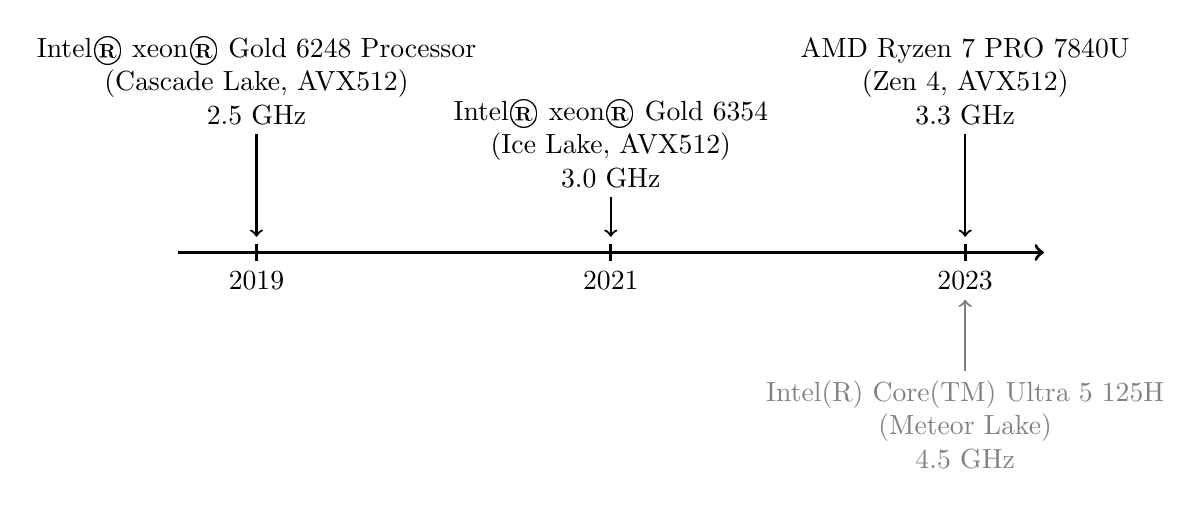
\begin{tikzpicture}[very thick, black]

    %coordinates
    \coordinate (O) at (1,0); % Origin
    \coordinate (F) at (12,0); %End
    \coordinate (P1) at (2,0); %ppti
    \coordinate (P2) at (6.5,0); %groebner
    \coordinate (P3) at (11,0); %mariz+argiope

    %proc
    \draw[<-,thick,color=black] ($(P1)+(0,0.2)$) -- ($(P1)+(0,1.5)$) node [above=0pt,align=center,black] 
    {Intel® xeon® Gold 6248 Processor \\ (Cascade Lake, AVX512) \\ 2.5 GHz};
    \draw[<-,thick,color=black] ($(P2)+(0,0.2)$) -- ($(P2)+(0,0.7)$) node [above=0pt,align=center,black] 
    {Intel® xeon® Gold 6354 \\ (Ice Lake, AVX512) \\ 3.0 GHz};
    \draw[<-,thick,color=black] ($(P3)+(0,0.2)$) -- ($(P3)+(0,1.5)$) node [above=0pt,align=center,black] 
    {AMD Ryzen 7 PRO 7840U \\ (Zen 4, AVX512) \\ 3.3 GHz};
    \draw[<-,thick,color=gray] ($(P3)-(0,0.6)$) -- ($(P3)-(0,1.5)$) node [below=0pt,align=center,gray] 
    {Intel(R) Core(TM) Ultra 5 125H \\ (Meteor Lake) \\ 4.5 GHz};

    %main arrow
    \draw[->] (O) -- (F);

    %ticks
    \foreach \x in {2,6.5,11}
    \draw(\x cm,3pt) -- (\x cm,-3pt);
    %labels
    \foreach \i \j in {2/2019,6.5/2021,11/2023}{
    	\draw (\i,0) node[below=3pt] {\j} ;
    }

\end{tikzpicture}

\bigskip
The processor marked in gray corresponds to a machine that does not provide AVX512 so it is only used to check the
correctness of the algorithms and will not appear in the timing comparisons of this document.

\begin{itemize}
    \item mention uops here ? allows to compare the performances 
\end{itemize}


\subsection{Vectorization}

\subsubsection{Auto-vectorization}

\textcolor{blue}{
\begin{itemize}
    \item auto-vec, flag \texttt{-O3}, help with loop unrolling
    \item \_\_attribute\_\_((optimize("-fno-tree-vectorize")))
\end{itemize}}

\subsubsection{Single Instruction Multiple Data}

The SIMD instructions of Intel form a set of assembly instructions that simultaneously perform an operation on multiple datas stored in registers
of a fixed size allowing to significantly improve the execution speed.

They are separated in families providing different operations on the basic types (int, long, float, double). We only used intrinsics from
the AVX2 and AVX512 sets.

\bigskip
All of the SIMD instructions have a name of the form:
\begin{center} 
    \texttt{<gen><prefix><op><type><size>}
\end{center}

where
\begin{center}
    \begin{minipage}{12cm}
        \begin{itemize}
            \item[\texttt{<gen>}] empty (SSE), v (AVX, AVX2, AVX512)
            \item[\texttt{<prefix>}] empty (unpacked), p (packed)
            \item[\texttt{<op>}] add, sub, mul, sl, sr, \dots
            \item[\texttt{<type>}] l (low part), h (high part), u (unsigned), s (signed), ss (signed with saturation)
            \item[\texttt{<size>}] b (byte - 8 bits), w (word - 16 bits), d (double word - 32 bits), q (quad word - 64 bits), 
            dq (double quad - 128 bits).
        \end{itemize}
    \end{minipage}
\end{center}


\begin{example}
    \texttt{vpmuludq} is an AVX instruction that multiplies the low unsigned 32-bit integers from packed 64-bit elements
    and store the unsigned 64-bit results.
\end{example}

\bigskip
Rather than directly use these instructions that would lead to writing assembly code, Intel proposes C-style functions
along with vector types that are accessible through the header \texttt{<immintrin.h>} and require the flag \texttt{-march=native} at 
compile-time.
They are described in the Intel intrinsics guide\footnote{\url{https://www.intel.com/content/www/us/en/docs/intrinsics-guide/index.html}}.

\bigskip
We mainly used two types of register: 
\begin{itemize}
    \item For AVX2: \texttt{\_\_m256i} which is a 256 bits register that can store up to 4 integers of 64 bits,
    \item For AVX512: \texttt{\_\_m512i} which is a 512 bits register that can store up to 8 integers of 64 bits,
\end{itemize}


\begin{example}
    The function \texttt{\_\_m256i \_mm256\_mul\_epu32(\_\_m256i a, \_\_m256i b)} performs the instruction \texttt{vpmuludq}
    on the 4 pairs of 64-bit integers stored in the registers a and b.
\end{example}

\subsection{Timings measurement}

Timings were measured using a profiling function that resembles the ones provided by FLINT.
It compares the different implementations of an operation for a given bit size of the modulus.

\bigskip
We have considered three ranges of sizes for the vectors:
\begin{itemize}
    \item small sizes: less than 200, 
    \item medium sizes: between 200 and 8000,
    \item large sizes: powers of two between $2^{13}=8192$ and $2^{22}=4194304$.
\end{itemize}

In some cases, timings obtained with small sizes and large sizes are not really conclusive because of
the mutiple load and store operations and the memory issues that can arise from the size of the caches.

\begin{remark}
    For basic operations, one can check the coherency of the timings by considering the clock speed of
    the processor used and the number of cycles it requires to complete the operation.
    
    For example, the Zen 4 processor has a clock speed of 3.3 GHz meaning it can handle about 
    3.3 billion cycles per second. Thus, considering the throughput of an operation performed on
    $N$ pairs of coefficients, we can expect a timing of about
    \[
    \dfrac{N\cdot throughput}{3.3\times 10^9}\quad \text{seconds}.
    \]

    This computation should only be used as an estimation since it does not take in account any
    delaying factors such as the latency.
\end{remark}

\bigskip
In theory, we could expect speed up factors of about 4 from the AVX2 intrinsics and of about 8 from the AVX512 intrinsics
since it corresponds to the number of pairs of coefficients they can handle simultaneously.
We will show that it is not particularly the case in practice.


\section{Multiplication of $64$-bit integers} 

When multiplying two integers, a problem of overflow can arise since the result might be too big to be stored in a $64$-bit word. 
To circumvent this issue, one needs to first split the two integers into two words of a given size and then apply the long multiplication.

\subsection{Long multiplication} \label{mulsplit}

The long multiplication consists in computing the multiplication of $64$-bit integers using multiplications and additions of
integers with a lower size.

\bigskip
Given two integers $x,y$ both of at most $64$ bits, we start by splitting them into 2 words, one of $k$ bits and the other one of at most $64-k$
bits with $k\leq32$:

\begin{align*}
    x &= x_{hi}\cdot 2^{k} + x_{lo} \\
    y &= y_{hi}\cdot 2^{k} + y_{lo}.
\end{align*}

\bigskip
We then compute:
\begin{align*}
    r_{lo} &= x_{lo}\cdot y_{lo} \\
    r_{mi} &= x_{lo}\cdot y_{hi} + x_{hi}\cdot y_{lo} \\
    r_{hi} &= x_{hi}\cdot y_{hi}
\end{align*}
and the final result is $ab = r_{lo} + (r_{mi} \ll k) + (r_{hi} \ll 2k)$. 
This formula is mathematically correct but is not used in practice since it would not fit in a $64$ bits word. 

\begin{remark}
    \
    \begin{itemize}
        \item For a value of $k$ lower than $32$, one has to check that each of the four products computed during the long multiplication can fit in a
        $64$-bit word, otherwise it can yield a wrong result.
        \item The addition involved in the computation of $r_{mi}$ can produce an overflow if the inputs are really up to $64$ bits.
        For this reason, we restrict the size of $x$ and $y$ to $63$ in practice. 
    \end{itemize}
\end{remark}

\subsection{Retrieve the high and the low part of the result}

Since the product $xy$ can have more than 64 bits, but always has at most 128 bits, the output of this operation is usually given as a pair of words of at most 64 
bits such that $xy = (xy)_{hi}\cdot 2^{64} + (xy)_{lo}$.

\bigskip
The exact formulas for these elements are:
\begin{align}
    (xy)_{lo} &= (r_{hi} \ll 2\cdot k) + (r_{mi} \ll k) + r_{lo} \nonumber \\
    (xy)_{hi} &= (r_{hi} \gg (64 - (2\cdot k))) + (r_{mi} \gg (64 - k)) + c \label{carry}
\end{align}
where $c$ corresponds to the carry coming from $(xy)_{lo}$.

\begin{remark}
    If one fixes $k=32$, then the above formulas can be slightly simplified:
    \begin{itemize}
        \item the shift left operation $(r_{hi} \ll 2\cdot k)$ will always yield 0,
        \item the shift right operation $(r_{hi} \gg (64 - (2\cdot k)))$ will always yield $r_{hi}$.
    \end{itemize}
\end{remark}

\bigskip
One can use the function \texttt{umul\_ppmm} provided by FLINT which is practical because it computes the product and
directly stores the 128-bit result before splitting it.
There are no such intrinsics in the AVX2 and AVX512 families.

\bigskip
In what follows, we consider the two operations:
\begin{itemize}
    \item \texttt{mullo(a,b)}: multiply the $x$-bit integers in $a$ and $b$, producing intermediate $2x$-bit integers, 
    and store the low $x$ bits of the intermediate integers.
    \item \texttt{mulhi(a,b)}: multiply the $x$-bit integers in $a$ and $b$, producing intermediate $2x$-bit integers, 
    and store the high $x$ bits of the intermediate integers.
\end{itemize}

In the AVX2 family, one can find intrinsics for \texttt{mullo} but only for integers up to 32 bits and intrinsics for 
\texttt{mulhi} but only for integers up to 16 bits.

In the AVX512 family, one can only find intrinsics for \texttt{mullo} (up to 64 bits) but they were rather slow
until recent processors such as ones of the Zen 4 generation.

\bigskip
\begin{table}[h!]
    \centering
    \begin{tabularx}{0.7\textwidth} { 
        | >{\centering\arraybackslash}X 
        | >{\centering\arraybackslash}X
        | >{\centering\arraybackslash}X 
        | >{\centering\arraybackslash}X | }
        \hline
        \rowcolor{myGray} 
        Processor & Cascade Lake & IceLake & Zen 4 \\
        \hline
        \cellcolor{myGray} Throughput & 1.5 & 3.0 & 1.0 \\
        \hline
    \end{tabularx}
    \caption{Throughputs of the instruction \texttt{vpmullq zmm, zmm, zmm} on different processors.}
\end{table}

Hence, we provide versions of the missing functions used in our implementations. They stick to the ones that can be found:
\begin{itemize}
    \item in the Vector Class library\footnote{\url{https://github.com/vectorclass/version2}} for \texttt{mullo} over 64-bit integers using AVX2,
    \item in the Intel HEXL library\cite{boemer2021intelhexlacceleratinghomomorphic} for \texttt{mulhi} over 64-bit integers using AVX512.
\end{itemize}
\textcolor{blue}{rewrite so that it doesn't seem like we just copy/pasted}

\subsection{Modular multiplications with precomputation}

In a context of several modular multiplications where one operand $w$ and the modulus $n$ are fixed,
V. Shoup\cite{Bos_Stam_2021} introduced a step of precomputation on $w$ and $n$ that will speed up subsequent multiplications by $w \mod n$.

\bigskip
Let $B$ be the maximum bitsize of a word ($B\in \{32, 64\}$). Given $n$ and $w \in \mathbb{Z}_n$, one can compute a scaled approximation 
of $\frac{w}{n}$, which is precisely $$ w_{pre} = \biggl\lfloor\dfrac{w\cdot 2^{B}}{n} \biggr\rfloor.$$

Then, for a vector $b = (b_1,\dots, b_N)$, one can compute $(w\cdot b_i \mod n)$ for each $i\in \{1, \dots, N\}$
using the following algorithm:

\begin{algorithm}
    \caption{Shoup modular multiplication}
    \begin{algorithmic}[1]
        \Require $n < 2^B$,
        \Require $0 < w < n$ and its precomputation $0 < w_{pre} < 2^B$,
        \Require $0 \leq b_i < n \qquad i\in \{1, \dots, N\}$.
        \Ensure $(w\cdot b_i \mod n)$.

        \State Compute $p_{hi}, p_{lo}$ such that $w_{pre} \cdot b_i = p_{hi}\cdot 2^B + p_{lo}$, \Comment{1 \texttt{mulhi}}
        \State $c \gets w\cdot b_i - p_{hi}\cdot n$ \Comment{2 \texttt{mullo}}
        \If {$c \geq n$}
            \State \Return $c-n$
        \Else
            \State \Return $c$
        \EndIf
    \end{algorithmic}
\end{algorithm}

\begin{remark}
    The branching at lines 3 to 7 satisfies:
    \[
    c \mod n = 
    \left\{
        \begin{array}{ll}
            c - n & \text{ if } c \geq n \\
            c & 
        \end{array}
    \right.
    = \min(c-n, c).
    \]
    Thus, using AVX512 intrinsics, one can use \texttt{\_mm512\_min\_epu64} to reduce $c$.
\end{remark}

\bigskip
The correctness of this algorithm relies on the definition of $w_{pre}$. 

\begin{proof} (Correctness of the algorithm)
First, we have that $w_{pre}= \left\lfloor\frac{w\cdot 2^B}{n}\right\rfloor $ is the quotient in the division 
of $w\cdot 2^B$ by $n$. Thus,
\[
    w\cdot 2^B = w_{pre}\cdot n + r \text{ with } 0 \leq r < n\ \Longleftrightarrow\ w_{pre} = \dfrac{w\cdot 2^B - r}{n}
\]

Then, by definition of $p_{hi}$,
\[
p_{hi} = \left\lfloor\frac{w_{pre}\cdot b_i}{2^B}\right\rfloor
= \left\lfloor\dfrac{w\cdot b_i}{n} - \dfrac{r\cdot b_i}{n\cdot 2^B} \right\rfloor.
\]

From the requirements on $r$ and $b_i$ and the previous result, we have that
\[
\left\lfloor\dfrac{w\cdot b_i}{n}\right\rfloor - 1 \leq p_{hi} \leq \left\lfloor\dfrac{w\cdot b_i}{n}\right\rfloor
\]
and this means that $p_{hi}$ is either $\left\lfloor\frac{w\cdot b_i}{n}\right\rfloor - 1$ or $\left\lfloor\frac{w\cdot b_i}{n}\right\rfloor$.


It follows that we have
\begin{align*}
\text{either } &c=w\cdot b_i - \left\lfloor\frac{w\cdot b_i}{n}\right\rfloor n + n = (w\cdot b_i \mod n)+n \\
\text{or } &c=w\cdot b_i - \left\lfloor\frac{w\cdot b_i}{n}\right\rfloor n = w\cdot b_i \mod n
\end{align*}
and the last step of the algorithm ensures that we retrieve $w\cdot b_i \mod n$.
\end{proof}

\begin{remark}
    In this particular case, one can omit the computation of the carry in equation (\ref{carry}) when performing the \texttt{mulhi} operation on $w_{pre}\cdot b_i$.

    If so, $p_{hi}$ might be off by one bit meaning that at the step 2 of the algorithm, we have 
    \[
    c = 
    \left\{
    \begin{array}{ll}
        & \ w\cdot b_i \mod n \\
        \text{or } & (w\cdot b_i \mod n) + n \\
        \text{or } & (w\cdot b_i \mod n) + 2n
    \end{array}
    \right.
    \]
    and the last case requires an additional substraction by $n$.

    This is the approach we used as it significantly speeds up the operation.
\end{remark}

\section{Classic arithmetic operations on vectors}

\textcolor{blue}{
    \begin{itemize}
        \item to get familiar with vectorization
    \end{itemize}
}

\subsection{Modular reduction}

Among the basic arithmetic operations, the modular reduction is one of the most costly. 
Thus, to circumvent its high cost, one can consider delaying it as long as there is no overflow occuring.
Another way is to modify the size requirements of the manipulated integers when the reduction boils down to
only a few additions or substractions.

These methods can't be applied on every operation. They will be more detailed when used.

\subsection{Addition of two vectors}

Given two vectors $a$, $b$ of $N$ coefficients in $\mathbb{Z}/n\mathbb{Z}$, we compute
\[
a_i + b_i \mod n \qquad \forall i\in \{1,\dots,N\}.
\]


\begin{remark}
    The modular reduction is done by only performing substractions and additions. It takes advantage of
    the fact that the sum of two integers $0 \leq x,y < n$ is less than $2n$.
\end{remark}

% 510, 2010, 32768
\begin{table}[h!]
    \centering
    
    % Proc 1: ppti
    \begin{tabular}{|r|*{3}{c c|}}
        \hline
        \rowcolor{myGray} 
        \multicolumn{7}{|c|}{\textsc{Cascade Lake}} \\
        \hline
        \rowcolor{myGray} 
         & 510 & & 2010 & & 32768 & \\
        \hline
        \cellcolor{myGray} Seq. & 4.89e-07 & 1.0x & 1.90e-06 & 1.0x & 3.17e-05 & 1.0x \\
        \hline
        \cellcolor{myGray} AVX2 & 1.26e-07 & 3.9x & 7.05e-07 & 2.7x & 1.43e-05 & 2.2x \\
        \hline
        \cellcolor{myGray} AVX512 & 8.17e-08 & 6.0x & 6.39e-07 & 3.0x & 1.27e-05 & 2.5x \\
        \hline
    \end{tabular}

    % Proc 2: groebner
    \begin{tabular}{|r|*{3}{c c|}}
        \hline
        \rowcolor{myGray} 
        \multicolumn{7}{|c|}{\textsc{Ice Lake}} \\
        \hline
        \rowcolor{myGray}
        & 510 & & 2010 & & 32768 & \\
        \hline
        \cellcolor{myGray} Seq. & xxxxxx & 1.0x & xxxxxx & 1.0x & xxxxxx & 1.0x \\
        \hline
        \cellcolor{myGray} AVX2 & xxxxxx & xxxx & xxxxxx & xxxx & xxxxxx & xxxx \\
        \hline
        \cellcolor{myGray} AVX512 & xxxxxx & xxxx & xxxxxx & xxxx & xxxxxx & xxxx \\
        \hline
    \end{tabular}

    % Proc 3: argiope
    \begin{tabular}{|r|*{3}{c c|}}
        \hline
        \rowcolor{myGray}
        \multicolumn{7}{|c|}{\textsc{Zen 4}} \\
        \hline
        \rowcolor{myGray}
        & 510 & & 2010 & & 32768 & \\
        \hline
        \cellcolor{myGray} Seq. & 2.60e-07 & 1.0x & 1.15e-06 & 1.0x & 1.76e-05 & 1.0x \\
        \hline
        \cellcolor{myGray} AVX2 & 6.04e-08 & 4.3x & 3.42e-07 & 3.4x & 6.71e-06 & 2.6x \\
        \hline
        \cellcolor{myGray} AVX512 & 6.04e-08 & 4.3x & 3.63e-07 & 3.2x & 6.25e-06 & 2.8x \\
        \hline
    \end{tabular}
    \caption{Timings in seconds and ratios of the modular sum with a 60-bit modulus.}
\end{table}

\begin{figure}[h!]
    \begin{center}
        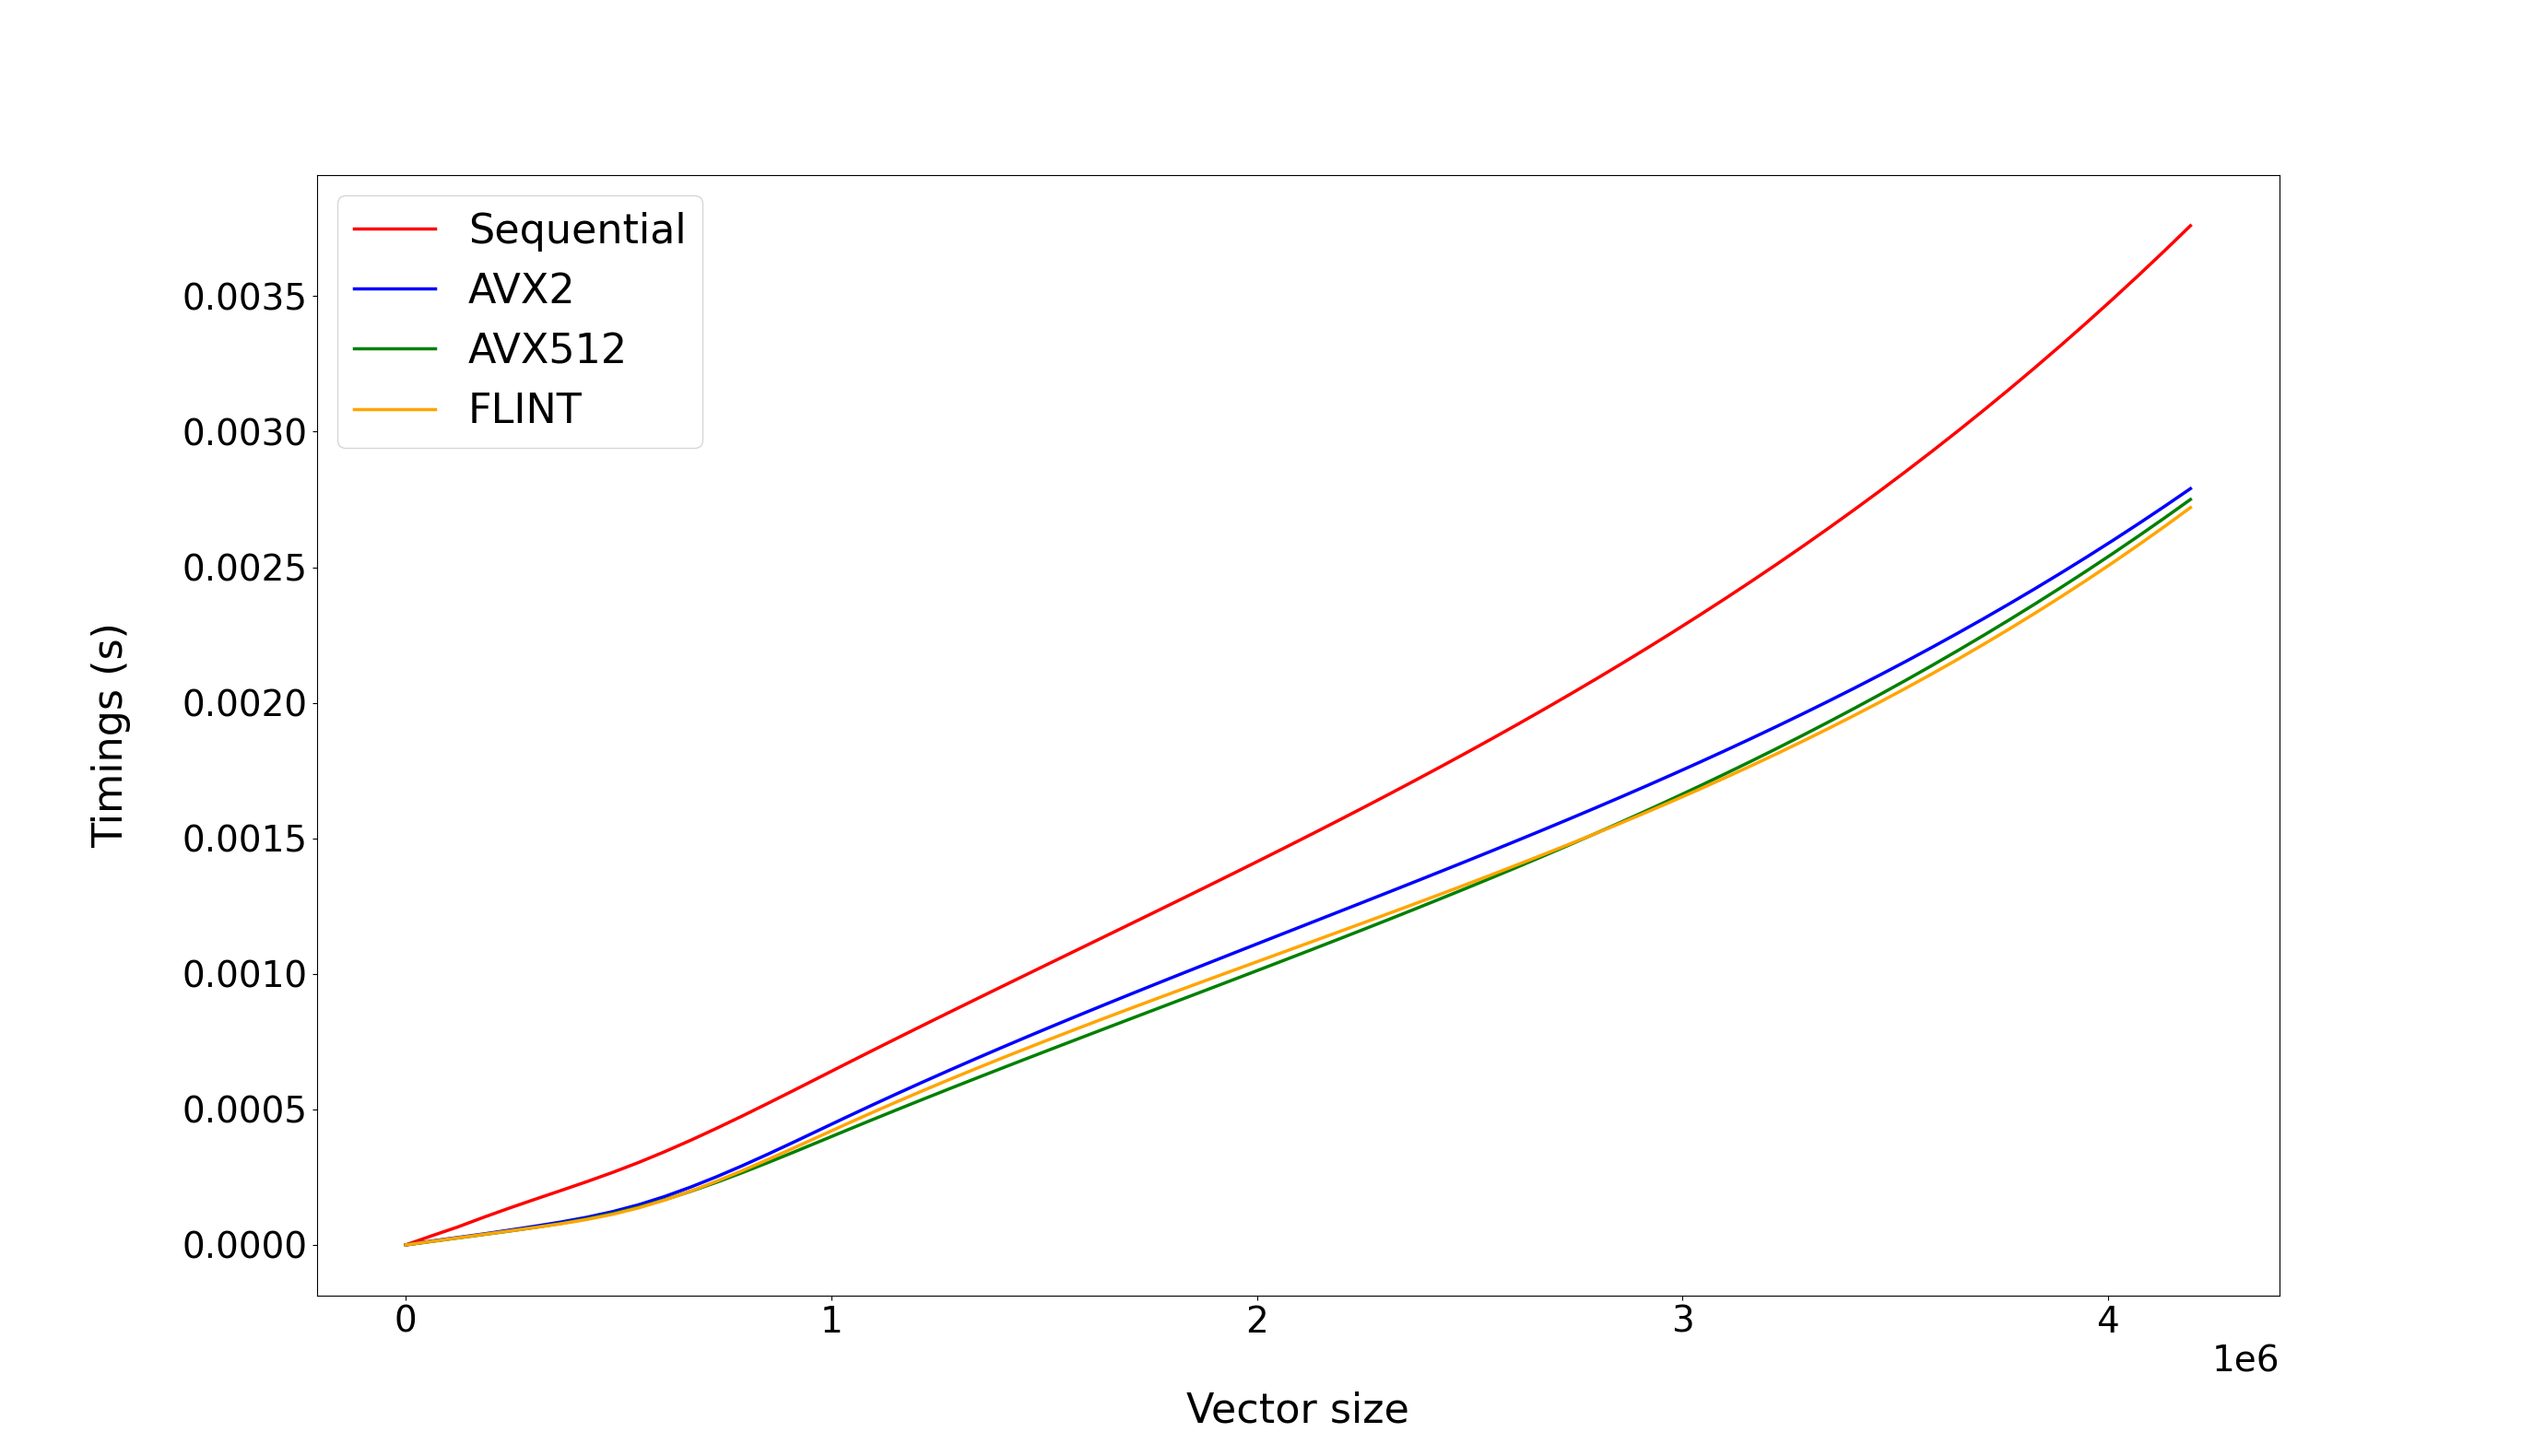
\includegraphics[width=0.8\textwidth]{add-mod_argiope.png}
    \end{center}
    \caption{Timings in seconds of the modular sum with a 60-bit modulus on a Zen 4 processor.}
\end{figure}

\newpage
\textcolor{blue}{
\begin{itemize}
    \item comment results
\end{itemize}}

\subsection{Multiplication of a vector by a scalar or by another vector}


\paragraph{Scalar-vector multiplication} Given a integer $w \in \mathbb{Z}/n\mathbb{Z}$ vector $b$ of $N$ coefficients in $\mathbb{Z}/n\mathbb{Z}$, we compute

\[
w \cdot b_i \mod n \qquad \forall i\in \{1,\dots,N\}.
\]

\paragraph{Element-wise vector-vector multiplication} Given two vectors $a$, $b$ of $N$ coefficients in $\mathbb{Z}/n\mathbb{Z}$, we compute
\[
a_i \cdot b_i \mod n \qquad \forall i\in \{1,\dots,N\}.
\]

\bigskip
These two operations share about the same properties and can both be implemented using the multiplication of 64-bit integers described 
in Section \ref{mulsplit}.

\begin{remark}
    None of the mentioned methods to bypass the modular reduction can be applied here. It has to be performed after each multiplication.
\end{remark}

We only show the results obtained with the scalar-vector product that was implemented using Shoup algorithm.

\textcolor{blue}{ timings +comments}

\subsection{Dot product}

Given two vectors $a,b$ of $N$ coefficients in $\mathbb{Z}/n\mathbb{Z}$, we compute
\[
\left(a_1\cdot b_1 + a_2\cdot b_2 + \dots + a_N\cdot b_N\right) \mod n = \left(\sum_{i=1}^N a_i\cdot b_i\right) \mod n.
\]

Each multiplication is performed by using the long multiplication of Section \ref{mulsplit} and then
the products are classically added together.
Like so, it requires to perform a reduction for each binary operation.

\bigskip
In fact, one can consider delaying the reduction according to the size of the modulus.
For instance, given a $k$-bit modulus, with $k < 32$, a product $a_i\cdot b_i$ fits in a word of 64 bits so
we can sum up to $2^{64 - 2k}$ terms before doing a reduction.

\begin{example}
    If $n < 2^{30}$, then $a_i\cdot b_i < 2^{60}$ for all $i$, and we can sum up to $2^4 = 16$ terms without any overflow:
    \[
    \forall i, \qquad a_i\cdot b_i < 2^{60}  
    \Longrightarrow \sum_{i=1}^{2^4} a_i\cdot b_i < \sum_{i=1}^{2^4} 2^{60} = 2^4 \cdot 2^{60} = 2^{64}.
    \]
\end{example}

\bigskip
This can also be applied with the results of long multiplications thus allowing $n$ to have a greater bit size.
In this case, we don't retrieve the high and low parts immediately, but instead
compute the sum of each $r_{lo}$, $r_{mi}$ and $r_{lo}$ computed like in section
\ref{mulsplit}. If we split at $l$ bits with $l \leq 32$, we end up with:
\begin{itemize}
    \item $r_{lo}$ of size $2 l$
    \item $r_{mi}$ of size $(k - l) + l + 1 = k$
    \item $r_{hi}$ of size $2 \left(k - l\right)$
\end{itemize}

Hence, we can sum up to
$2^{64 - \max\left(2 l, k + 1, 2 \left(k - l\right)\right)}$ terms without
overflow.

% TODO:
% - label for sec 2

\begin{remark}
    The size of the result is not a limit for the number of term we can sum.
    This result is stored in 128 bits in total, so if $k \in \{2, \dots, 64\}$ is
    the size of the terms, up to $2^{128 - 2k}$, which is higher than the
    previous value.
\end{remark}

\textcolor{blue}{
    \begin{itemize}
        \item timings + comments
        \item Speak a little bit more about reconstruction and mod?
    \end{itemize}
}

\section{Butterfly Fast Fourier Transform}

The butterfly refers to an operation that takes place in Cooley-Tukey algorithm \cite{Cooley_Tukey_1965}, a common algorithm to perform 
Fast Fourier Transform (FFT), which takes as inputs: $n, w$ a modulus and a scalar of at most 64 bits, and two integers 
$x, y$ in $\mathbb{Z}_n$, and performs the in-place computation:
\[
(x,y) \mapsto (x + w\cdot y \mod n,\ x - w\cdot y \mod n).
\]

Looking at the more global picture, in the FFT algorithm such a butterfly will
be applied to a long vector of different \(x_i, y_i\) but with the same \(w\) and \(n\).


\subsection{Harvey lazy butterfly FFT}

Harvey proposes a strategy\cite{DBLP:journals/corr/abs-1205-2926} to compute the butterfly FFT base on Shoup multiplication
with the precomputation step that allows to save two
modular reductions compared to a basic implementation if one is able to restrict the sizes of the modulus. 

\begin{algorithm}
    \caption{Harvey lazy butterfly FFT}
    \begin{algorithmic}[1]
        \Require $n < 2^B/4$,
        \Require $0 < w < n$ and its precomputation $0 < w_{pre} < 2^B$,
        \Require $0 \leq x, y < 4n$.
        \Ensure $(x,y) \mapsto (x + w\cdot y \mod n,\ x - w\cdot y \mod n), \qquad 0 \leq x,y < 4p.$

        \If {$x \geq 2n$}
            \State $x \gets x - 2n$
        \EndIf
        \State Compute $p_{hi}, p_{lo}$ such that $w_{pre} \cdot y = p_{hi}\cdot 2^B + p_{lo}$ \Comment{1 \texttt{mulhi}}
        \State $t \gets w\cdot y - p_{hi}\cdot n$ \Comment{2 \texttt{mullo}}
        \If {$t \geq 2n$}
            \State $t \gets t - 2n$
        \EndIf
        \State $x \gets x + t$
        \State $y \gets x - t + 2n$
        \State \Return $x,y$
    \end{algorithmic}
\end{algorithm}

\textcolor{blue}{
    \begin{itemize}
        \item explain this is our version, and one can find a similar one in hexl
        \item timings + comments
    \end{itemize}
}


\section{Conclusion}

Altogether, the results are rather conclusive and we can hope for them to be later used in FLINT. 

\bigskip
To have a more complete study, we could have looked at the case in which the modulus is a prime number
with a particular form such as the ones presented in the appendix \ref{app}. 

This is possible in the context of the FFT, and could have enhance the butterfly FFT even more.

\bigskip
Another possible improvement is to use the Integer Fused Multiply Add Instructions (IFMA) that are part of
the AVX512 family. This extension provides some intrinsics with a low throughput for operations that involve
multiplications and additions but requires to lower the maximum bit size allowed to 52. \textcolor{blue}{$\Rightarrow$floating-point arithmetic}


\newpage
\bibliographystyle{plain} 
\bibliography{biblio} 
\nocite{*}


\newpage
\appendix
\section{Modular reduction with special primes} \label{app}

\subsection{Mersenne numbers}

\begin{definition}
    A Mersenne number is of the form $$ M_n = 2^n-1,$$ where $n$ is an integer.

    If $n$ is prime, $M_n$ is also prime and is therefore called a Mersenne prime.
\end{definition}

From this special form, we have for any $n$,
\[
M_n = 0 \mod M_n \Longleftrightarrow 2^n = 1 \mod M_n.
\]

Thus, any integer $x < M_n^2$ can be reduced modulo $M_n$ using only one addition: 
\begin{align*}
x \mod M_n &= x_{hi}\cdot 2^{n} + x_{lo} \mod M_n \\
    &= x_{hi} + x_{lo} \mod M_n.
\end{align*}


\subsection{Generalized Mersenne primes}

Following the same idea presented with Mersenne primes, one can expect to be able to significantly simplify
the modular reduction using generalized Mersenne primes of the form:
\begin{align*}
    p &= 2^u + 2^v + 1 \\ 
    p &= 2^u - 2^v + 1 
\end{align*}
of $u+1$ bits, with $64 > u > v > 0$.

This needs a further analysis to be conclusive.

\end{document}
